\documentclass{config/apuntes}

\title{Algoritmos en Bioinformática}
\author{Sandra Mingo Ramírez}
\date{2024/25}
\acronym{ALGBIO}

\usepackage[all]{nowidow}
\usepackage{listing}
\usepackage{color}
\usepackage{tabularx}
\usepackage{multirow}
\usepackage{makecell}
\usepackage{amsmath}
\usepackage{array}

\definecolor{dkgreen}{rgb}{0,0.6,0}
\definecolor{gray}{rgb}{0.5,0.5,0.5}
\definecolor{mauve}{rgb}{0.58,0,0.82}

\lstset{
  language=Python,
  frame=tb,
  aboveskip=3mm,
  belowskip=3mm,
  showstringspaces=false,
  columns=flexible,
  basicstyle={\small\ttfamily},
  numbers=none,
  numberstyle=\tiny\color{gray},
  keywordstyle=\color{blue},
  commentstyle=\color{dkgreen},
  stringstyle=\color{mauve},
  breaklines=true,
  breakatwhitespace=true,
  tabsize=3
}

\begin{document}

\begin{abstract}
En bioinformática se necesita aplicar conocimientos para resolver problemas en nuevos contextos. Además, se necesita capacidad de elaborar proyectos de investigación o aplicaciones en bioinformática, incorporando soluciones innovadoras, anticipando dificultades y valorando estrategias alternativas de contingencia, así como consideraciones en cuanto a responsabilidad social, ética y legal. Para ello, es imprescindible conocer y manejar los principales métodos de algoritmia y su aplicación en bioinformática. Concretamente, nos centraremos en las estructuras de datos, la notación O y órdenes de ejecución, la búsqueda y ordenación, la programación dinámica y aplicaciones algorítmicas en bioinformática para la búsqueda de perfiles y alineamientos.
\end{abstract}

\pagestyle{plain}

\maketitle

\tableofcontents

%examen final 50%
%entrega prácticas y ejercicios 50%
%BLOQUES
%Introducción a algoritmos y estructura de datos -> miniproject y examen a realizar desde casa y entregar
%Programación dinámica
%Trayectorias eulerianas y secuenciación del ADN
%Técnicas de diseño de algoritmos aplicadas a la búsqueda de motivos y alineamiento de secuencias

%28/01 - José Dorronsoro
\chapter{Introducción a los algoritmos y estructuras de datos}
\section{Algoritmos y estructura de datos}
Un programa es el resultado de la \textbf{ecuación de Wirth}, es decir, la suma de algoritmos y estructura de datos.

\subsection{Algoritmos}
Los algoritmos tienen muchas definiciones, pero ninguna es muy precisa. Wikipedia define los algoritmos como "un conjunto de reglas que definen con precisión una secuencia de operaciones para realizar alguna tarea y que finalmente se detienen". Normalmente, están escritos en \textbf{pseudocódigo}, algo intermedio entre lenguaje natural y código de ordenador. Los tres bloques principales de un algoritmo son:
\begin{itemize}
\item \textbf{Bloque secuencial:} bloques de sentencias (ordinarias) que se ejecutan secuencialmente en su totalidad. Las sentencias pueden tener sólo cómputos directos o varias llamadas a funciones. El orden de ejecución es según la ley de la gravedad. En Python, se definen como bloques formados por sentencias con la misma sangría.
\item \textbf{Selecciones:} sentencias en las que la ejecución se bifurca a diferentes bloques según alguna condición. En Python se reconoce en bloques if, elif y else.
\item \textbf{Repeticiones o loops:} un bloque de sentencias se repite mientras se cumpla alguna condición. Puede haber un bucle for para un cierto número de repeticiones o un bucle while si hay una condición.
\end{itemize}

\subsection{Ejemplo: Algoritmo de Euclid}
El algoritmo de Euclid calcula el máximo común divisor de dos números positivos a, b calculando repetidamente r = a\%b y sustituyendo a por b y b por r mientras r > 0 (siendo r el resto). En Python:
\begin{lstlisting}
def euclid_gcd(a, b):
	while b > 0:
		r = a % b
		a = b
		b = r
		#Alternativa pitónica: a, b = b, a % b
		
	return a
\end{lstlisting}

La ecuación de Wirth es bonita y correcta en general, pero los programas también necesitan bastante \textbf{manejo de excepciones}, es decir, detectar situaciones excepcionales y decir al programa qué hacer cuando se producen. Los errores de argumentos son fáciles de prevenir y de manejar. Las excepciones de ejecución, cosas que van mal durante la ejecución, son más difíciles de detectar y prevenir. La programación debe ser muy \textbf{defensiva}.

\subsection{Estructura de datos}
Los algoritmos trabajan con datos. Variables individuales están bien para algoritmos simples. Las estructuras de datos son formas de organizar datos complejos para algoritmos avanzados. Las estructuras de datos más simples son strings, listas y arrays, las avanzadas son diccionarios y sets, y las más avanzadas listas enlazadas, árboles y grafos, aunque estos últimos están disponibles por la importación de módulos.

\subsubsection{Strings, listas, arrays y diccionarios}
Los elementos de strings, listas y arrays son accesibles mediante índices, mientras que los diccionarios están compuestos por parejas clave:valor. Todos son objetos de Python con atributos, variables con información del objeto, y métodos, funciones que actúan sobre el contenido del objeto. \texttt{dir(objeto)} lista todos los atributos y métodos del objeto.

\subsubsection{Listas enlazadas}
Las listas enlazadas están compuestas por nodos con campos \texttt{data} que contienen la información del nodo y \texttt{next} que apunta al siguiente nodo. Son una versión dinámica de los arrays, y son útiles cuando el número de nodos y/o su localización no se conoce previamente.

\begin{figure}[htbp]
\centering
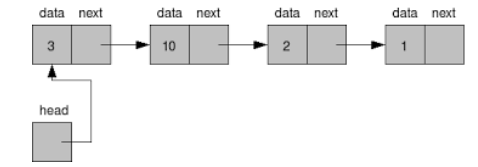
\includegraphics[width = 0.5\textwidth]{figs/linked-lists.png}
\end{figure}

\subsubsection{Árboles}
Los árboles contienen nodos de datos organizados de forma jerárquica con un único nodo raíz y los demás tienen un padre y quizás hijos.

\begin{figure}[htbp]
\centering
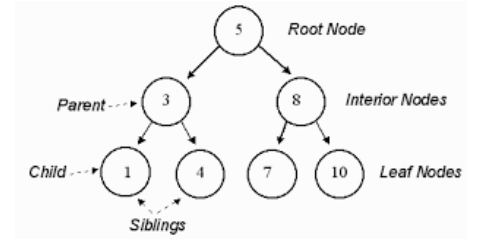
\includegraphics[width = 0.5\textwidth]{figs/tree-datastructure.png}
\end{figure}

\subsubsection{Grafos}
Los grafos están compuestos por nodos o vértices conectados por edges. Posiblemente es la estructura de datos más general: puede representar mapas de carreteras, redes sociales, interacciones de proteínas, etc.

\begin{figure}[htbp]
\centering
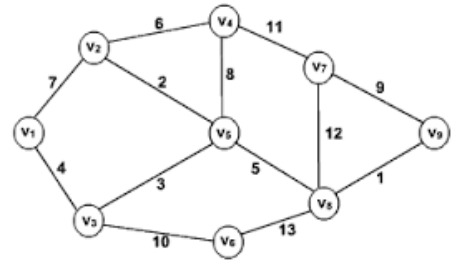
\includegraphics[width = 0.5\textwidth]{figs/graph-datastructure.png}
\end{figure}

\section{Diseño de algoritmos}
La escritura de algoritmos (y la programación en general) suele hacerse ad hoc. Es un acto creativo: debe seguir las reglas de programación pero también requiere imaginación, creatividad y experiencia. Lo mismo ocurre con la escritura ordinaria, ya que no podemos llenar una página vacía sólo con reglas gramaticales. La programación también requiere trabajo duro, mucha práctica y, además, bastante lectura de algoritmos. A veces podemos aprovechar las técnicas generales de diseño derivadas de una larga experiencia en resolución de problemas y análisis de algoritmos. No pueden aplicarse como reglas empíricas automáticas, pero pueden tener un amplio rango de aplicabilidad. Consideraremos tres: \textbf{algoritmos codiciosos}, \textbf{algoritmos de divide y vencerás} (también conocidos como \textbf{recursivos}) y \textbf{programación dinámica}.

\subsection{El problema del cambio - algoritmo codicioso}
Supongamos que tenemos trabajo como cajero y nuestros clientes quieren cambio en el menor número de monedas posible. ¿Cómo podemos proceder? La idea más sencilla: dar a cada paso la moneda más grande y más pequeña que la cantidad que queda por cambiar. Ejemplo: ¿cómo dar cambio de 3,44 euros? Fácil: una moneda de 2 euros, una moneda de 1 euro, dos monedas de 20 céntimos, dos monedas de 2 céntimos. Hay que escribir el algoritmo pero la idea general es codiciosa: Intentamos minimizar \textbf{globalmente} el número total de monedas, pero lo hacemos \textbf{localmente} usando en cada paso la moneda más grande posible para minimizar la cantidad que queda por cambiar.

Suponiendo que trabajamos con monedas/billetes de 1, 2, 5, 10, 20, 50, 100 y 200, queremos guardar el número de monedas/billetes de cada tipo a devolver en un diccionario:
\begin{lstlisting}
def change(c):
	assert c >= 0, "change for positive amounts only"
	l_coin_values = [1, 2, 5, 10, 20, 50, 100, 200]
	d_chainge = {}
	
	for coin in sorted(l_coin_values) [::-1]:
		d_change[coin] = c//coin
		c = c%coin
		
	return d_change
\end{lstlisting}

Aparentemente, esto funciona. Pero si debemos dar un cambio de 7 con monedas 1, 3, 4 o 5, la respuesta más eficiente solo requiere dos monedas, una de 4 y una de 3, pero este algoritmo cogería una de 5 y tendrá que dar dos monedas de 1. Esto ocurre bastante con algoritmos codiciosos: son muy naturales, pero pueden dar una respuesta equivocada. La forma de resolver esto sería con programación dinámica.

\subsection{Las torres de Hanoi - algoritmo recursivo}
Se nos da un conjunto de 64 discos de oro de diferentes tamaños apilados en la pila A en tamaños crecientes, y otras dos pilas vacías B, C. Queremos mover la primera pila a B un disco cada vez usando C como clavija auxiliar obedeciendo la regla de que ningún disco puede colocarse encima de otro disco más pequeño. Esto es fácil para 2 discos, no muy difícil para 3, pero para 4 la dificultad aumenta. 

Se puede obtener una solución recursiva sencilla para N discos. Primero se mueven los primeros N-1 discos de la pila A a la C utilizando B como pila auxiliar. El disco restante se mueve de A a B. Los N-1 discos restantes se mueven de C a B usando A como pila auxiliar. 
\begin{lstlisting}
def hanoi(n_disks, a=1, b=2, c=3):
	assert n_disks > 0, "n_disks at least 1"
	
	if n_disks == 1:
		print("Move disk from %d to %d" % (a,b))
	else:
		hanoi(n_disks - 1, a, c, b)
		print("move disk from %d to %d" % (a,b))
		hanoi(n_disks - 1, c, b, a)
\end{lstlisting}

Con esto, hay que tener cuidado con los tiempos de ejecución incluso para n\_disks pequeños. De hecho, el problema general de Hanoi es extremadamente costoso incluso para un número moderado de discos.

Los algoritmos recursivos suelen derivar de una estrategia de «divide y vencerás»: Dividir un problema P en M subproblemas $P_m$, resolverlos por separado obteniendo soluciones $S_m$ y combinar estas soluciones en una solución S de P.

En el caso de las torres de Hanoi se pueden dividir dos subproblemas: P1 es el subproblema de mover N - 1 discos de A a C usando B, y P2 el subproblema de mover N - 1 discos de C a B usando A. Se pueden combinar los movimientos según el código de Python. Los algoritmos son eficientes si los subproblemas son sustancialmente más pequeños - pero esto no es el caso de Hanoi.

\section{Eficiencia de algoritmos}
En primer lugar, los algoritmos deben ser correctos, ya que un algoritmo rápido, pero erróneo, es inútil.  También es deseable que no requieran (mucha) memoria extra. La función \texttt{hanoi} cumple esto: sólo se usan sus parámetros. Algo a tener en cuenta en bioinformática, ya que los datos pueden ser muy grandes, es que también es muy deseable que los algoritmos sean lo más rápidos posible. Pero un algoritmo debe leer sus entradas, y si hay muchas y grandes, esto ralentizará el algoritmo. No obstante, los tiempos de ejecución deseables no deberían estar muy por encima del \textbf{mismo orden de magnitud que el tamaño de sus entradas}.

\subsection{Estimar tiempos de ejecución}
En primer lugar, no se miden solo los tiempos reales, ya que dependen del lenguaje, la máquina, el programador y, por supuesto, las entradas. Por tanto, dependen demasiado del contexto para permitir generalizaciones significativas. En su lugar, hay que centrarse en \textbf{tiempos abstractos} medidos contando las \textbf{operaciones clave} que el algoritmo realiza en una entrada dada. Para los algoritmos iterativos, normalmente se busca la operación clave en el bucle más interno. Contando cuántas veces se realizan estas operaciones clave se obtiene una buena estimación del tiempo que tardarán los algoritmos. De esta forma, el coste del algoritmo de cambio viene dado por la longitud de la lista de monedas.

El análisis de algoritmos recursivos es (mucho) más difícil. Para Hanoi, la operación clave puede ser \texttt{print("move disk from \%d to \%d" \% (a, b))}, pero aunque aparece explícitamente en el código, también tiene lugar dentro de las llamadas recursivas. Esto da lugar a estimaciones recurrentes del coste de los algoritmos recursivos que a menudo son difíciles de escribir y resolver. Se pueden desarrollar algunas estrategias generales en algoritmos mucho más sencillos basados en bucles. 

\subsection{Multiplicación de matrices}
Un algoritmo muy conocido y relativamente costoso es $c_{i,j} = \sum^n_{k=1} a_{i,k}b_{k,j}$. Un código de Python simple y malo que describe esto es el siguiente:
\begin{lstlisting}
def matrix_multiplication(m_1, m_2):
	n_rows, n_interm, n_columns = m_1.shape[0], m_2.shape[0], m_2.shape[1]
	m_product = np.zeros( (n_rows, n_columns) )
	
	for p in range(n_rows):
		for q in range(n_columns):
			for r in range(n_interm):
				m_product[p, q] += m_1[p, r] * m_2[r, q]
				
	return m_product
\end{lstlisting}

Aquí, la operación clave es \texttt{m\_1[p, r] * m\_2[r, q]}. Asumiendo matrices cuadradas con N filas y columnas, esta operación clave se repite $N \times N \times N = N^3$, lo cual es sustancialmente más grande que el tamaño del problema $N^2 + N^2 = 2N^2$.

%04/02 
\subsection{Búsqueda lineal}
Para buscar una clave en una lista, lo más sencillo es comparar la clave con todos los elementos de la lista hasta que se encuentre. 
\begin{lstlisting}
def linear_search(key, l_ints):
	for i, val in enumerate(l_ints):
		if val == key:
			return i
				
	return None
\end{lstlisting}

En este caso, la operación clave es \texttt{if val == key}. Encontrar la clave que esté en \texttt{l\_ints[0]}, solo se requiere una operación, pero para \texttt{l\_ints[-1]}, se requieren \texttt{N = len(l\_ints)} operaciones, al igual que si la clave no se encuentra en la lista.

\subsection{Notación o, O y $\Theta$}
Dado un algoritmo, y sabiendo la operación básica, hay una función que calcula el coste de dicha operación. La multiplicación de matrices tiene un coste $f_{MM} (N) = N^3$, y la búsqueda lineal $f_{LS}(N) = N$. Por tanto, se pueden comparar dos algoritmos mediante la comparación de su función de coste.  

Suponemos que las funciones de coste son positivas y crecientes (así deberían ser los tiempos de ejecución abstractos de los algoritmos)

Se dice que $f = o(g)$ si ambas son positivas en el tiempo ($\frac{f(N)}{g(N)} \rightarrow 0$), y el crecimiento de $f$ es considerablemente menor que el de $g$.

Además, $f = O(g)$ si encontramos una constante C de un entero N que depende de C de manera que $f(N) \leq Cg(N)$ siempre que $N \geq N_C$. De esta forma, $g$ será eventualmente mayor que $f$ con la ayuda de $C$.

Finalmente, $f = \Theta(g)$ si $f = O(g)$ y $g = O(f)$. 

En resumen, y de manera informal, podemos decir:
\begin{itemize}
\item $f < g$ cuando $f = o(g)$
\item $f \leq g$ cuando $f = O(g)$
\item $f \approx g$ cuando $f = \Theta(g)$ y, por tanto, $g = \Theta(f)$
\end{itemize}

Por ejemplo, antes definimos unas funciones con coste $N^2$ y $N^3$. Al hacer $\frac{N^2}{N^3} = \frac{1}{N}$, tendiendo N a infinito, el resultado es 0, por lo que $N^2 = o(N^3)$. Además, como $N^2 \leq 1 \cdot N^3$, entonces también $N^2 = O(N^3)$, pero esto es menos preciso.

\subsection{Complejidad de un algoritmo}
A partir de un algoritmo A con un input I, se puede medir el tiempo de ejecución abstracto de la siguiente forma:
\begin{itemize}
\item Podemos identificar la operación clave en A y estimar su trabajo abstracto en I siguiendo el número $n_A(I)$ de veces que A se ejecuta en I.
\item Se puede asignar un tamaño N al input I
\item Podemos encontrar una función $f_A(N)$ de forma que $n_A(I) = O(f_A(N))$
\end{itemize}
En algunos casos, esto se puede refinar a $n_A(I) = \Theta(f_A(N))$. Por tanto, $f_A(N)$ da la complejidad de A sobre las entradas de tamaño N. Para el problema de Hanoi, tenemos $n_{Hanoi}(N) = 2^N - 1$. En las búsquedas lineales, aquellas búsquedas exitosas son $n^e_{LS}(N) \leq N$, pero también puede darse $n^e_{LS}(N) = 1$, por lo que el peor escenario de la búsqueda lineal es $W(N) = N$, ya que siempre $n_{LS}(k, l_ints) \leq N$.

\subsection{De tiempos abstractos a tiempos reales}
En Python, está el comando \texttt{\%timeit} que permite la estimación de tiempos de ejecución en el caso de funciones simples. 
\begin{lstlisting}
a = np.ones((100, 100))
b = np.eye(100)
%timeit -n 10 -r 1 matrix_multiplication(a, b)
\end{lstlisting}
Si \texttt{timeit} nos devuelve 1s (para 100 elementos), en el caso de matrices de 500 podemos esperar $500 = 5 \times 100, 500^3 = 125 \times 100^3$, es decir, 125 segundos. Esto no es muy preciso, pero sirve para una estimación. Hay que tener en cuenta que librerías grandes como \texttt{numpy} o \texttt{pandas} utilizan C o C++ para el código compilado al ser más rápido.
%04/02 - José Dorronsoro
\chapter{Programación dinámica}
\section{Revisando el problema del cambio}
Volvemos al problema de devolver el cambio de una cantidad de dinero. El algoritmo codicioso no siempre llegaba a la solución más óptima en cuanto a menor número de monedas devueltas. 
En este caso, el truco está en descomponer el problema en subproblemas y crear una fórmula para ir de un subproblema al siguiente.

Suponiendo que debemos dar un cambio C y tenemos las monedas $v_1 = 1, \ldots v_n$, entonces $n(i, c)$ es el número mínimo de monedas a cambiar utilizando solo las primeras $i$ monedas. Lo que queremos es $n(N, C)$, que se obtiene del subproblema $n(i, c)$. Además:
$$n(i,0) = 0$$
$$n(1,c) = c$$

Con esto, se puede rellenar una matriz con las monedas como filas y el posible cambio como columna. Para rellenar la posición $n(i,c)$:
\begin{itemize}
\item Si la moneda $i$ no entra en el cambio: $n(i - 1, c)$
\item Si la moneda $i$ sí entra en el cambio: $1 + n(i, c - v_i)$
\end{itemize}

\subsection{El algoritmo del cambio en programación dinámica}
De esta forma, llegamos a
$$n(i, c) = min{n(i - 1, c), 1 + n(i, c - v_i)}$$
con un coste $O(1)$.

En el problema, queríamos dar un cambio de 7 con monedas 1, 3, 4 y 5: $n(4, 7)$ Para ello, tenemos una tabla con las filas 1, 3, 4 y 5 y las columnas 0 1 2 3 4 5 6 7. La primera fila, con la moneda de 1, se rellena con el valor del cambio que hay que dar. Para la fila del 3, los valores de las columnas 0 1 y 2 se mantienen como la fila anterior, ya que no se puede utilizar esta moneda para un cambio menor a su valor. A partir del valor de la moneda, se debe retroceder ese valor en número de columnas y sumarle 1. Ese valor hay que compararlo con el de la celda justamente superior, y ver el valor mínimo, el cual se mantiene. Siguiendo esta lógica, llegamos a que el número de monedas mínimo para este problema son 2.

\begin{figure}[h]
\centering
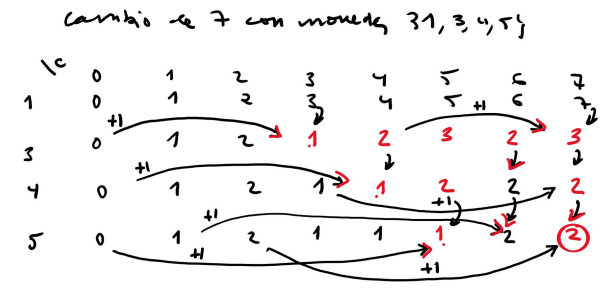
\includegraphics[width = 0.7\textwidth]{figs/dp-cambio.png}
\end{figure}

En este caso, hemos calculado $7 (c) \times 4 (n) = 28$ veces. El coste de un algoritmo sin bucles es constante: $f(n) = 1$. Por tanto, en este caso el coste es $28 \times O(1)$, y de forma general:
$$N \times C \times O(1) = O(N \times C) = O(N \times 2^{logC})$$
siendo $2^{logC}$ el logaritmo binario de C (los bits en los que se puede codificar).

\section{Algoritmos de cadenas en programación dinámica}
Para un informático, una secuencia biológica son cadenas de texto.
Teniendo dos cadenas, para transformar una en la otra, se puede:
\begin{itemize}
\item Cambiar un caracter por otro
\item Insertar un caracter
\item Borrar un caracter
\end{itemize}
Insertar un caracter en una cadena es equivalente a borrar un caracter en la otra. Además, queremos mantener una cadena constante y modificar solo la otra. 

La \textbf{distancia de edición} entre dos cadenas es el número mínimo de de operaciones de edición que se deben hacer para convertir una en la otra. 

Dados los strings S y T con M y N número de caracteres respectivamente,se consideran los substrings  
$$S_i = [s_1, \ldots s_i]$$
$$T_i = [t_1, \ldots t_j]$$

Así, $d_{i,j}$ es la distancia de edición entre $S_i$ y $T_i$. Si $s_i = t_j$, entonces $d_{i,j} = d_{i-1, j-1}$, ya que la diferencia se encuentra antes. Si $s_i \neq t_j$, hay tres opciones:
\begin{itemize}
\item Cambiar $t_j$ por $s_i$; entonces $d_{i,j} = 1 + d_{i-1, j-1}$
\item Borrar $t_j$ de $T_j$; entonces $d_{i,j} = 1 + d_{i, j-1}$
\item Borrar $s_i$ de $S_i$; entonces $d_{i,j} = 1 + d_{i-1, j}$
\end{itemize}
De estas tres opciones, se calculan todas y nos quedamos con el mínimo.

\subsection{Rellenar la matriz}
Tenemos una matriz con M filas y N columnas. Esto se multiplica por lo que cuesta calcular cada elemento, O(1): $O(M \times N)$. Esto es caro en tiempo y en memoria. 

Finalmente, tenemos las siguientes ecuaciones para el problema de la distancia de edición:
$$d_{i,j} = \begin{cases}
d_{i-1, j-1} & \text{cuando} s_i = t_j \\
1 + min {d_{i-1, j-1}, d_{i, j-1}, d_{i-1, j}} & \text{cuando} s_i \neq t_j
\end{cases} $$

Ejemplo: encontrar la distancia de edición entre \texttt{biscuit} y \texttt{suitcase}.
\begin{figure}[h]
\centering
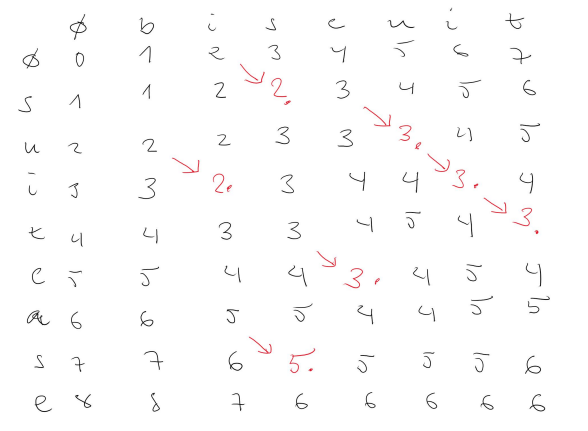
\includegraphics[width = 0.6\textwidth]{figs/edit-distance-ex.png}
\end{figure}

No obstante, en biología, se asignan costes a cambiar y a borrar diferentes dependiendo del caso.

%11/02 - José Dorronsoro
\chapter{Eulerian, Hamilton y Secuenciación de ADN}
\section{Caminos eulerianos y hamiltonianos}
\subsection{Teoría de grafos - Ejemplo de Königsberg}
\subsubsection{Caminos eulerianos}
Un \textbf{grafo} es una estructura matemática compuesta por un conjunto de \textbf{vértices} (o nodos) y un conjunto de \textbf{aristas} (o ramas) que conectan pares de vértices. Las aristas pueden ser \textbf{dirigidas} (con una dirección específica) o \textbf{no dirigidas} (sin dirección). En una representación gráfica, los vértices se representan como puntos y las aristas como líneas que los conectan.

\begin{figure}[h]
\centering
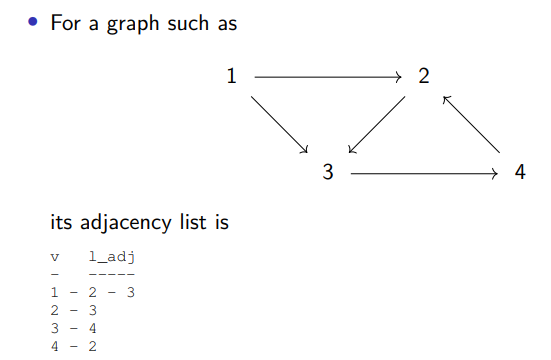
\includegraphics[width = 0.8\textwidth]{figs/graph.png}
\end{figure}

En un grafo, el \textbf{grado de entrada} (in degree) de un vértice es el número de aristas que llegan a él, mientras que el \textbf{grado de salida} (out degree) es el número de aristas que salen de él. En grafos no dirigidos, el grado de un vértice simplemente se refiere al número de aristas incidentes a él.

\subsubsection{El Problema de los Puentes de Königsberg}
El problema de los puentes de Königsberg es un famoso problema matemático que data del siglo XVIII. La ciudad de Königsberg (actualmente Kaliningrado) estaba dividida por el río Pregel, con dos islas conectadas entre sí y con las orillas del río mediante siete puentes. El desafío consistía en encontrar un camino que permitiera cruzar cada puente exactamente una vez y regresar al punto de partida.

Este problema puede modelarse como un \textbf{grafo no dirigido}, donde cada región de la ciudad (orillas e islas) se representa como un vértice, y cada puente como una arista que conecta dos vértices. El objetivo es encontrar un \textbf{camino euleriano}, es decir, un recorrido que pase por cada arista exactamente una vez.

\subsubsection{Condiciones para la Existencia de Caminos Eulerianos}
Un \textbf{camino euleriano} es un recorrido que atraviesa cada arista de un grafo exactamente una vez. Si el camino comienza y termina en el mismo vértice, se denomina \textbf{circuito euleriano}.

Para que un grafo no dirigido tenga un camino euleriano, se deben cumplir las siguientes condiciones:
\begin{itemize}
\item El grafo debe estar conectado (es decir, debe existir un camino entre cualquier par de vértices).
\item Exactamente dos vértices deben tener un grado impar. Estos vértices serán el punto de inicio y el punto final del camino.
\item Todos los demás vértices deben tener un grado par.
\end{itemize}

En el caso de un circuito euleriano, todas las condiciones anteriores se mantienen, excepto que todos los vértices deben tener un grado par, ya que el camino debe comenzar y terminar en el mismo vértice.

\subsubsection{Aplicación al Problema de Königsberg}
En el grafo que representa los puentes de Königsberg, todos los vértices tienen un grado impar. Por lo tanto, no es posible encontrar ni un camino euleriano ni un circuito euleriano. Esto llevó a Leonhard Euler a concluir que no existe una solución al problema original.

Euler no solo demostró que estas condiciones son necesarias, sino también suficientes. Es decir, si un grafo no dirigido cumple las condiciones mencionadas, entonces existe un camino o circuito euleriano.

\subsubsection{Observaciones Adicionales}
En un circuito euleriano, el punto de partida es irrelevante, ya que el recorrido terminará en el mismo vértice. Sin embargo, no todos los puntos de partida permiten recorrer todas las aristas en un camino euleriano que no sea un circuito.

En grafos dirigidos, las condiciones para la existencia de caminos eulerianos son análogas, pero deben considerarse los grados de entrada y salida de cada vértice.

\subsubsection{Caminos hamiltonianos}
Si G es un grafo no dirigido, un camino hamiltoniano es un camino en G que visita cada nodo sólo una vez. Mientras que los caminos eulerianos tenían un coste de $O(|E|)$, encontrar un camino hamiltoniano es mucho más costoso computacionalmente. 

\subsection{Secuenciación del ADN hamiltoniana y euleriana}
El objetivo de la secuenciación del genoma es descomponer un gen en una secuencia de cuatro letras (A, T, G, C). 
A grandes rasgos, la secuenciación Shotgun sigue un proceso de cuatro pasos:
\begin{enumerate}
\item Dividir el gen en lecturas cortas aleatorias de 100-500 bases.
\item Identificar las secuencias de lectura hibridándolas en una micromatriz de ADN.
\item Reconstruir cada lectura a partir de estas secuencias.
\item Reconstruir el gen completo a partir de las lecturas.
\end{enumerate}
Los primeros dos pasos son bioquímica pura, pero el tercer paso se basa en caminos hamiltonianos o eulerianos. 

La hibridación de microarrays funciona de la siguiente forma:
\begin{itemize}
\item Colocar todas las sondas de longitud $l$ posibles, es decir, secuencias de ADN de una longitud $l$ fija, en los puntos de una micromatriz.
\item Colocar una gota de ADN marcado con fluorescencia en cada micropunto de la matriz.
\item El fragmento de ADN se hibrida con las micropuntos que son complementarias a una determinada subsecuencia de longitud $l$ del fragmento. De esta forma obtenemos todas las posibles subsecuencias de longitud $l$ que forman el fragmento pero están desordenadas. Siguen el orden en el microarray pero no el de la secuencia.
\end{itemize}

Llamamos $l$-mero a la secuencia de cada una de las sondas. El $l$-espectro sp(S, $l$) de una secuencia S es el conjunto de todos los $l$-meros de S. Por ejemplo, para S = [TATGGTGC] tenemos sp(S, 3)= {TAT, ATG, TGG, GGT, GTG, TGC}. Después de la hibridación, las sondas hibridadas en el microarray nos dan una versión desordenada de sp(S, $l$) que tenemos que reordenar para recuperar S. Definimos el solapamiento $\omega(s1,s2)$ entre dos $l$-mers s1, s2 como la longitud más larga de un sufijo de s1 que también es un prefijo de s2. Claramente tenemos $\omega(s1,s2) \leq l - 1$. Ahora, si s2 sigue a s1 en S, debemos tener $\omega(s1,s2) = l - 1$.

Se puede reconstruir la secuencia S encontrando y ordenando $s_{i1} \ldots s{ik}$ de $sp(S, l)$ de forma que $\omega(s_{ij}, s{ij+1}) = l - 1$. Esto sugiere definir un grafo $G_l(S) = (V_l, E_l)$ donde $V_l = sp(S, l)$ y $(s, s') \in E_l$ si $\omega(s, s') = l - 1$.
Reconstruir S es equivalente a pasar una vez por todos los nodos de $G_l(S)$. De esta formal, podemos reconstruir S encontrando un camino hamiltoniano en $G_l(S)$.
\begin{figure}[h]
\centering
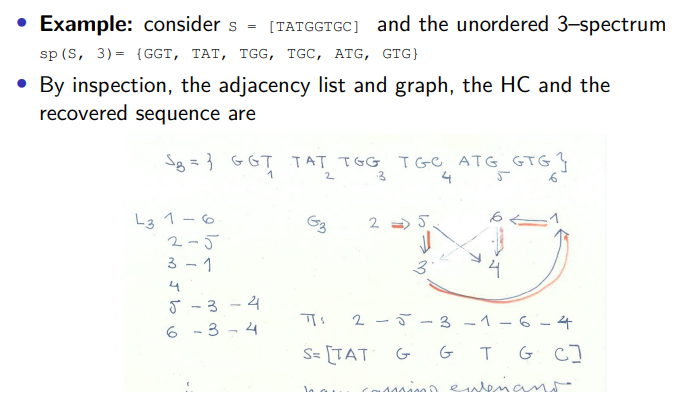
\includegraphics[width = \textwidth]{figs/hamiltonian-dna.png}
\end{figure}

El problema de los caminos hamiltonianos es que son algoritmos muy poco eficientes. La alternativa es intentar hacer $l$-meros en los vértices en lugar de en los nodos. Si $s \in sp(S, l)$ y $\delta_1$ es el prefijo de $l - 1$ y $\delta_2$ su sufijo, podemos considerar s como el vértice que conecta los nodos $\delta_1$ y $\delta_2$. De esta forma tenemos $\omega(\delta_1, \delta_2) = l - 2$. Ahora, podemos definir el grafo $G_{l-1} = (V_{l-1}, E_{l-1})$ donde $V_{l-1} = sp(S, l-1)$ y $(\delta, \delta') \in E_{l-1}$ si son respectivamente prefijo y sufijo de $s \in sp(S, l)$. De esta forma, reconstruir S es equivalente a pasar una vez por todos los vértices de $G_{l-1}$: encontrar el camino euleriano.

Este grafo es dirigido, por lo que hay que adaptar la teoría del camino euleriano a este tipo de grafos. En un grafo dirigido $G(V, E)$ tenemos que distinguir entre vértices incidentes y adyacentes. Por cada $u \in V$, decimos que $(u, v)$ es un vértice adyacente para u e incidente para v. 

\begin{figure}[h]
\centering
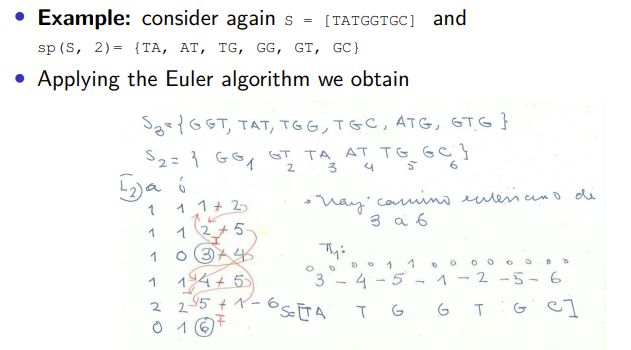
\includegraphics[width = \textwidth]{figs/eulerian-dna.png}
\end{figure}

\chapter{Resumen complejidad algorítmica}
\begin{table}[h]
\centering
\begin{tabular}{l l }
\multicolumn{2}{c}{O: Peor caso} \\ \hline
$O(1)$ & \texttt{def constante(arr): return arr[0]} \\ 
$O(n)$ & \texttt{for x in arr: print(x)} \\ 
$O(n^k)$ & \texttt{for i in range(n):} \\ 
 & \texttt{\ \ for j in range(n): print(arr[i], arr[j])} \\ 
$O(\log n)$ & \texttt{while n > 1: n //= 2} \\ 
$O(\log \log n)$ & \texttt{while n > 2: n = log2(n)}  \\ 
$O(n \log n)$ & \texttt{merge\_sort(arr)} \\ 
\end{tabular}
\end{table}

\begin{table}[h]
\centering
\begin{tabular}{l l }
\multicolumn{2}{c}{o: Límite superior no ajustado} \\ \hline
$o(1)$ & No aplica (es constante) \\ 
$o(n)$ & \texttt{for i in range(sqrt(n)): print(i)}\\ 
$o(n^k)$ & \texttt{for i in range(n):} \\ 
 & \texttt{\ \ for j in range(log(n)): print(i, j)} \\ 
$o(\log n)$ & \texttt{while n > 1: n = sqrt(n)}  \\ 
$o(\log \log n)$ & \texttt{while n > 2: n = log2(log2(n))}  \\ 
\end{tabular}
\end{table}

\begin{table}[h]
\centering
\begin{tabular}{l l }
 \multicolumn{2}{c}{$\Theta$: Límite ajustado} \\ \hline
$\Theta(1)$ & \texttt{def constante(arr): return arr[0]} \\ 
$\Theta(n)$ & \texttt{for x in arr: print(x)} \\ 
$\Theta(n^k)$ & \texttt{for i in range(n):} \\ 
& \texttt{\ \ for j in range(n): print(arr[i], arr[j])} \\ 
$\Theta (\log n)$ & \texttt{while n > 1: n //= 2} \\ 
$\Theta (\log \log n)$ & \texttt{while n > 2: n = log2(n)} \\ 
$\Theta(n \log n)$ & \texttt{merge\_sort(arr)} \\ 
\end{tabular}
\end{table}
%20/02 - Ana González Marcos
\chapter{Aplicación de algoritmos a problemas bioinformáticos}
La búsqueda de motivos se realiza mediante búsqueda exhaustiva, algoritmos codiciosos o algoritmos aleatorios. Los algoritmos de programación dinámica se emplean para los alineamientos. Un motivo es una secuencia específica y corta que aparecen frecuentemente en una región del ADN o secuencia proteica. Representa una región conservada en secuencias que suelen tener significado biológico. 

\section{Búsqueda exhaustiva}
La búsqueda exhaustiva es la única búsqueda "de verdad" que da una solución determinista exacta. También se conoce como búsqueda por fuerza bruta. El algoritmo examina todas las posibles alternativas para encontrar una solución óptima. El tiempo de cómputo es muy alto, pese a que requiera de poco esfuerzo en su diseño. Como las secuencias biológicas son muy largas, este tipo de búsquedas es inviable. 
En el patrón se busca encontrar un consenso que se puede representar gráficamente en logos. 

Una posible aplicación es la búsqueda de un patrón de x nucleótidos (x-mer) sin mutaciones. También se pueden incorporar un par de mutaciones y generar un consenso. Con esto se calcula el perfil y se ve cuántos nucleótidos caen en cada posición. Se busca el perfil que, aun con mutaciones, da un motivo consenso. 

El consenso es un motivo ancestro del cual surgen los motivos mutados. Para calcular la medida que indique lo buen consenso que es un motivo, se tiene en cuenta la homología, es decir, la similitud debida a un ancestro común. La distancia entre un motivo real y la secuencia de consenso suele ser menor que la de dos motivos reales. Necesitamos introducir una función de puntuación para comparar diferentes conjeturas (consenso) y elegir la «mejor». 
$$Score(s, DNA) = \sum^l_{i = 1} \max_{k \in A T G C} count(k, i)$$

Se busca a lo largo de todas las cadenas, desde la primera posición el tamaño del l-mer. En definitiva, el algoritmo es:
\begin{lstlisting}
BruteForceMotifSearch(DNA, t, n, l)
bestScore = 0
for each s=(s1, s2, ..., st) from (1, 1 ... 1) to (n-l + 1, ..., n-l + 1)
	if Score(s, DNA) > bestScore
		bestScore = score(s, DNA)
		bestMotif = (s1, s2, ... st)
return bestMotif
\end{lstlisting}

Como esta búsqueda es exhaustiva, para $(n - l + 1)$ posiciones en t secuencias, se buscan $(n - l + 1)^t$ sets de posiciones iniciales. Para cada posición inicial, la función de puntuación hace $l$ operaciones, de forma que la complejidad es:
$$l \cdot (n - l + 1)^t \rightarrow O(l \cdot n^t)$$
De esta forma, hay veces en las que no es posible hacer este cálculo.

\subsection{Median String}
El median string es la alternativa a la búsqueda exhaustiva. En este caso se busca en las secuencias un patrón. No se utiliza la puntuación de antes, si no que utiliza la distancia de Hamming. La distancia de Hamming entre dos mer se define como el número de nucleótidos distintos entre ellos. 
$$d_H(AAAAAA, ACAAAC) = 2$$
$$d_H(v, s) = \sum^t_{i = 1} d_H(v, s_i)$$
Antes se buscaba la puntuación máxima, pero ahora buscamos la distancia mínima. 

\begin{lstlisting}
MedianStringSearch(DNA, t, n, l)
bestWord = AAAAA...A
bestDistance = infinity
for each l-mer v from AAA...A to TTT...T
	if TotalDistance(v, DNA) < bestDistance:
		bestDistance = TotalDistance(v, DNA)
		bestWord = v
return bestWord
\end{lstlisting}

La búsqueda de motivos es un problema de maximización, mientras que la cadena mediana es un problema de minimización. Sin embargo, el problema de la Búsqueda de Motivos y el de la Cadena Mediana son computacionalmente equivalentes. Hay que demostrar que minimizar TotalDistance es equivalente a maximizar la puntuación.

Con este algoritmo, la complejidad es de $4^l$. El coste es considerablemente más bajo que en la búsqueda exhaustiva, ya que el tamaño del mer es más pequeño que el tamaño de la secuencia. Por tanto, reformular un problema puede ayudar a disminuir la complejidad computacional. 

%25/02 - Ana
\section{Algoritmo codicioso}
Un algoritmo codicioso es un algoritmo que siempre toma la mejor solución inmediata, o local, mientras encuentra una respuesta.
Los algoritmos codiciosos:
\begin{itemize}
\item a menudo devuelven resultados subóptimos, pero tardan poco en hacerlo.
\item seleccionan la alternativa «más atractiva» en cada iteración.
\item suelen ser heurísticas rápidas que cambian precisión por velocidad para encontrar una solución aproximada/subóptima.
\end{itemize}

En este caso, se utiliza la entropía como medida. Es una medida probabilística que se suele definir como $\int -p \log (p)$. Está la entropía sobre todos los nucleótidos se correspondería a $- \sum p \cdot \log_2(p)$. Esto se utiliza para calcular los logos. Motif logo es un diagrama para visualizar la conservación de motivos que consiste en una pila de letras en cada posición. La altura total de cada columna se basa en el contenido informativo de la columna, que se define como $2 - H_i(p_A, p_C, p_G, p_T)$. Cuanto menor es la entropía, mayor es el contenido de información, lo que significa que las columnas altas del logotipo del motivo están muy conservadas. 

La probabilidad del l-mer es la probabilidad de que un l-mer a fuese creado por el perfil P:
$$p(a|P) = \Pi^l_{k=1} P_{a_{i,k}}$$ 
donde $P_{a_{i,k}}$ es la probabilidad de la letra $a_i$ en la posición $k$, distribuida independientemente e idénticamente. 

\begin{lstlisting}
GreedyMotifSearch(DNA, k, t)
BestMotifs = primer k-mer de cada string de ADN
for each k-mer Motif in the first string in DNA do
	Motif1 = Motif
	for i = 2 to t do
		form Profile from Motif1, ..., Motif i-1
		Motif i = profile-most probable k-mer in the ith string in DNA
	Motifs = Motif i, ..., Motif t
	if Score(Motif) > Score (BestMotif) then
		BestMotifs = Motifs
return BestMotifs
\end{lstlisting}

Primero, se inicializa una matriz de motivos con los primeros -lmers de cada secuencia de ADN. Después se va comparando el l-mer de la primera secuencia con la siguiente secuencia, calculando el mejor motivo, el cual se añade a una nueva lista. Así se recorren las distintas secuencias. Tras obtener la lista de los motivos (uno por cada secuencia), se obtiene el consenso. Éste se puntúa y se compara con la puntuación de la matriz inicializada, quedándonos con la matriz que tenga una puntuación mayor. A continuación se mueve el primer l-mer un nucleótido y repetir todo este proceso.

Para evitar obtener resultados de 0, se utiliza la regla de sucesión de Laplace, sumando 1 a todos los valores de contaje para computar las probabilidades mediante pseudo-counts. De esta forma, se obtiene la matriz del perfil. 

En cuanto al tiempo del cómputo, como tenemos una matriz $t \times n$ de ADN y una longitud del patrón $l$, el tiempo de ejecución es $O(n^2 \cdot l \cdot t)$, lo cual es mejor que el algoritmo de fuerza bruta. No obstante, es restrictivo, por lo que podemos no encontrar los mejores motivos. Cambiando el orden de las secuencias, el resultado va a ser distinto, afectando significativamente el rumbo que tomará el análisis. 

\section{Algoritmos randomizados}
Los algoritmos aleatorios toman decisiones aleatorias en lugar de deterministas. Estos algoritmos se utilizan en situaciones en las que no se conoce ningún algoritmo polinómico correcto. Seleccionan aleatoriamente posibles ubicaciones y encuentran una forma de cambiar codiciosamente esas ubicaciones hasta que hayamos convergido al motivo oculto.

\begin{lstlisting}
RandomizedMotifSearch(DNA, l, t)
Randomly select l-mers Motifs = (Motif1, ... Motift) in each string from DNA
BestMotifs = Motifs
while forever
	Profile = PROFILE(Motifs)
	Motifs = MOTIF(Profile, DNA)
	if Score(Motifs) > Score(BestMotifs)
		BestMotifs = Motifs
	else
		return BestMotifs
\end{lstlisting}

Este algoritmo se detiene tras un número de iteraciones que le demos, o cuando el perfil apenas se modifique tras más iteraciones. El algoritmo se ejecuta muchas veces, cada una de ellas con nuevos l-mers inicializados, y con la colección de los motivos con mayor puntuación se obtiene el consenso. 

\subsection{Gibbs Sampling}
RandomizedMotifSearch puede cambiar todas las cadenas $t$ en Motifs en una única iteración. Puede sondear imprudentemente, y algunos motivos correctos pueden ser descartados en la siguiente iteración.

GibbsSampler es un algoritmo iterativo más cauteloso que descarta un único $l$-mers del conjunto actual de motivos en cada iteración y decide conservarlo o sustituirlo por uno nuevo. Los pasos son:
\begin{enumerate}
\item Elegir aleatoriamente las posiciones iniciales de l-mers para cada secuencia.
\item Elegir al azar una de las secuencias $t$
\item Crear un perfil $P$ (consenso) a partir de las otras secuencias ($t - 1$)
\item Para cada posición de la secuencia eliminada, se calcula la probabilidad de que el $l$-mer que comienza en esa posición haya sido generado por $P$.
\item Elegir al azar una nueva posición inicial para la secuencia eliminada basándose en las probabilidades calculadas en el paso anterior.
\end{enumerate}

Este proceso se itera hasta dar con la solución, es decir, que la puntuación no mejore más. 
GibbsSampler funciona bien en muchos casos. Dado que GibbsSampler explora sólo un pequeño subconjunto de soluciones, puede «atascarse» en un óptimo local. Al igual que RandomizedMotifSearch, debe ejecutarse varias veces con la esperanza de que una de estas ejecuciones produzca los motivos con mejor puntuación.

Estos algoritmos aleatorizados funcionan porque el ADN no es del todo aleatorio, conteniendo motivos reguladores que permiten un control preciso sobre la expresión genética. Estos motivos resultan en un perfil esperado sesgado.

%27/02
\section{Algoritmo divide-y-vencerás}
En estos algoritmos, el problema se divide en subproblemas, conquistándolos de forma recursiva. Si los subproblemas son lo suficientemente pequeños, se resuelven de forma bruta. Las soluciones de los subproblemas se deben combinar en una solución para el problema original, siendo esto lo complicado. Un algoritmo de divide y vencerás hace más trabajo del necesario, resolviendo repetidamente los subproblemas comunes. 

\section{Programación dinámica}
La programación dinámica se basa en la premisa de calcular primero las soluciones a subproblemas más pequeños y utilizarlas después para resolver problemas sucesivamente más grandes hasta obtener la respuesta. La programación dinámica se utiliza cuando se podría recurrir a la recursividad, pero sería ineficaz porque resolvería repetidamente los mismos subproblemas. Se toma un problema que podría resolverse recursivamente de arriba abajo y, en su lugar, se resuelve iterativamente de abajo arriba. Los resultados intermedios se almacenan en una tabla para su uso posterior; de lo contrario, se acabarían calculando repetidamente, lo que constituye un algoritmo ineficaz.

Por ejemplo, la programación dinámica se utiliza para ver la similitud entre genes. El alineamiento de secuencias es esencial para filogenia, análisis genómico, predicción de genes, estructura proteica, estructura de ARN secundario, búsqueda en bases de datos, etc. Si los alineamientos son erróneos, todos los resultados basados en los alineamientos están mal.

En el alineamiento de secuencias se distingue el alineamiento por pares, donde se alinean dos secuencias, del alineamiento múltiple, donde se utilizan más de dos secuencias. 

\subsection{Problema de la subsecuencia común más larga}
Los biólogos que encuentran una nueva secuencia genética suelen querer saber con qué otras secuencias es más parecida. Encontrar una subsecuencia es una forma de calcular el grado de similitud entre dos secuencias: cuanto más larga es la subsecuencia, más similares son. Los caracteres de una subsecuencia, a diferencia de los de una subcadena, no tienen por qué ser contiguos.

\subsection{Matriz de sustitución}
El problema del ADN es que puede mutar: mutación puntual de un nucleótido, inserción o deleción. Encontrar la similitud del ADN es importante, ya que secuencias similares pueden tener funciones similares. Uno de los algoritmos más ampliamente utilizados es BLAST. 

La matriz de puntuación de sustitución es una matriz bidimensional con valores de puntuación que describen la probabilidad de que un aminoácido o nucleótido haya sido reemplazado durante la evolución de la secuencia. Se pueden penalizar la apertura de huecos y la mutación puntual, creando una matriz ponderada. Se da una puntuación positiva a los pares de caracteres idénticos o similares y una puntuación negativa a los diferentes. Esta puntuación se basa en las frecuencias observadas de tales ocurrencias en alineaciones de ADN/proteínas relacionadas evolutivamente.

El parámetro más crítico en la comparación de secuencias es la elección de una matriz de puntuación/sustitución. Para una evolución reciente, se suele utilizar una matriz de identidad, ya que se espera que las secuencias no hayan divergido mucho. Para una evolución antigua, la matriz converge a un modelo aleatorio. En bioinformática hay varias matrices: PAM, BLOSUM, Gonnet, JTT.

\subsection{Matrices de puntuación}
\paragraph{PAM}
PAM viene de Point Accepted Mutation. Contiene la probabilidad derivada empíricamente de que se acepte una sustitución, basada en proteínas estrechamente relacionadas. Los números PAM más altos corresponden a una mayor distancia evolutiva. Cuando dos secuencias tienen una diferencia de 1 PAM, significa que una secuencia se puede transformar en la otra con una media de mutaciones puntuales de un 1\% (una mutación por cada 100 aminoácidos).

\paragraph{BLOSUM}
BLOSUM viene de Blocks Substitution Matrix. Es otra matriz derivada empíricamente, basada en proteínas relacionadas a mayor distancia. Los números BLOSUM más bajos corresponden a una mayor distancia evolutiva.

La comparación entre PAM y BLOSUM, a un nivel comparable de sustituciones, indica que los dos tipos de matrices producen resultados similares

\subsection{Needleman-Wunsch - alineamiento global}
Este método realiza un alineamiento global entre dos secuencias. Se inicializa en 0, y se rellena la matriz con el valor máximo entre la mutación puntual o el hueco (ya sea en una secuencia o en la otra) mediante la matriz de puntuación. 

\begin{figure}[h]
\centering
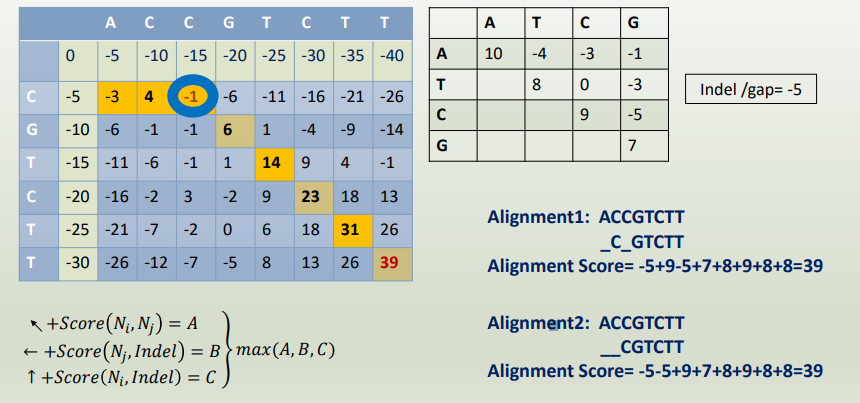
\includegraphics[width = 0.8\textwidth]{figs/needleman-wunsch.png}
\end{figure}

Una vez calculada la matriz F, la esquina inferior derecha de la matriz es la puntuación máxima de cualquier alineación. Para calcular qué alineación da realmente esta puntuación, se puede empezar por la celda inferior derecha y comparar el valor con las tres fuentes posibles (Opción1, Opción2 y Opción3) para ver de cuál procede.
\begin{itemize}
\item Si es la opción 1, entonces las dos secuencias están alineadas.
\item Si es la opción 2, entonces la primera secuencia está alineada con un hueco.
\item Si es la opción 3, entonces la segunda secuencia está alineada con un hueco.
\end{itemize}

El alineamiento global suele utilizarse para alinear secuencias que tienen aproximadamente la misma longitud y que ya se sabe que están relacionadas.

\subsection{Smith-Waterman - alineamiento local}
En este caso, se busca la mejor puntuación de los alineamientos de regiones de secuencias. De esta forma, se encuentran segmentos conservados, en lugar de alinear la secuencia completa. La diferencia con Needleman-Wunsch es la posibilidad de coger 0 como posibilidad a la hora de rellenar la matriz.

\begin{figure}[h]
\centering
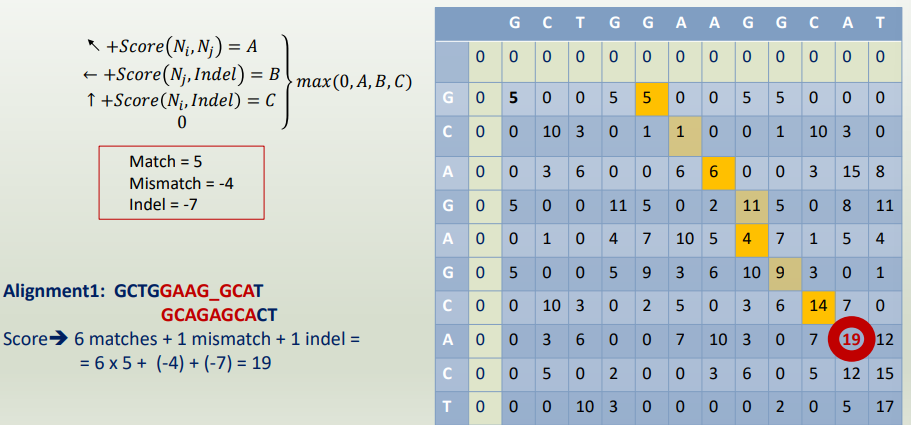
\includegraphics[width = 0.8\textwidth]{figs/smith-waterman.png}
\end{figure}

Tanto el algoritmo de Needleman-Wunsch como el de Smith-Waterman utilizan los conceptos de matriz de sustitución/puntuación, función de penalización por hueco y proceso de rastreo. 

\begin{table}[h]
\begin{mdframed}[backgroundcolor=black!10]
\textbf{Ejercicio:} encuentra el mejor alineamiento local entre TCAGTTGCC y AGGTTG con +1 para match, -2 para mistmatch y -2 para gap.

\begin{tabular}{c c c c c c c c c c c}
&&T&C&A&G&T&T&G&C&C\\
&0&0&0&0&0&0&0&0&0&0\\
A &0 &0&0&1&0&0&0&0&0&0\\
G &0 &0&0&0&2&0&0&0&0&0\\ 
G &0 &0&0&0&3&1&0&2&0&0\\ 
T &0 &1&0&0&1&4&1&3&1&0\\ 
T &0 &2&0&0&0&5&5&6&2&0\\ 
G &0 &0&0&0&2&1&3&6&5&3\\ 
\end{tabular}

Por tanto, la parte común es GTTG.

\textbf{Ejercicio:} lo mismo que antes, pero para el mejor alineamiento global.
\begin{tabular}{c c c c c c c c c c c}
&&T&C&A&G&T&T&G&C&C\\
&0&-2&-4&-6&-8&-10&-12&-14&-16&-18\\
A &-2 &-2&-4&-3&-5&-7&-9&-11&-13&-15\\
G &-4 &-4&-6&-5&-2&-4&-6&-8&-10&-12\\ 
G &-6 &-6&-8&-7&-4&-3&-5&-5&-7&-9\\ 
T &-8 &-4&-6&-7&-5&-2&-2&-4&-6&-8\\ 
T &-10 &-6&-6&-8&-6&-3&-1&-3&-5&-7\\ 
G &-12&-8&-8&-8&-5&-5&-3&0&-2&-4\\ 
\end{tabular}
Por tanto, el resultado es:\\
TCAGTTGCC\\
AG-GTTG
\end{mdframed}
\end{table}

%04/03 - Ana
\section{Búsqueda en bases de datos}
El tiempo de búsqueda en grandes bases de datos es una consideración importante, y se hace necesario equilibrar la velocidad y la sensibilidad de la búsqueda. Los métodos exhaustivos, como Needleman-Wunsch y Smith-Waterman, suelen garantizar una respuesta óptima, pero tardan demasiado en comparar una secuencia con una base de datos. En un intento de ganar velocidad con una pérdida aceptable de sensibilidad, se han derivado métodos aproximados a partir de estos algoritmos.

\subsection{Métodos heurísticos}
Los métodos heurísticos para buscar en una base de datos son:
\begin{itemize}
\item FastA: Primer algoritmo rápido de búsqueda de secuencias para comparar una secuencia de consulta con una base de datos
\item BLAST: Es una mejora de FastA en cuanto a velocidad de búsqueda, facilidad de uso, rigor estadístico y sensibilidad.
\end{itemize}

Tanto FASTA como BLAST buscan similitud local entre secuencias.

\subsubsection{FastA}
FastA es un algoritmo de varios pasos para el alineamiento de secuencias. Primero se buscan regiones de dos secuencias que parezcan prometedoras, es decir, que tengan algún grado de similitud. Después se computa el alineamiento local usando programación dinámica en estas regiones. Si simplemente se comparan dos secuencias cualesquiera para ver si son homólogas, Smith-Waterman sería el método a elegir. Las características de FastA son:
\begin{itemize}
\item Alineamiento local: intenta encontrar parches de similitud regional, en lugar de tratar de encontrar el mejor alineamiento entre toda la secuencia query y las secuencias de la base de datos. 
\item Alineamiento con gaps: los alineamientos generados pueden contener huecos.
\item Rapidez: es un método heurístico, pudiendo perder coincidencias. Así, no hay garantía de encontrar el mejor alineamiento. Utiliza una estrategia que sacrifica la sensibilidad completa para ganar velocidad.
\end{itemize}

La programación dinámica calcula la puntuación en un montón de zonas inútiles para encontrar secuencias subóptimas. Se buscan secuencias cortas en las que haya matches. Normalmente, en el ADN se busca con una longitud de 6 nucleótidos y para proteínas 2 aminoácidos. 
Los pasos del algoritmo son:
\begin{enumerate}
\item Identificar k-meros comunes entre las secuencias I y J.

Los k-meros comunes se representan en un dot matrix. Cada elemento tiene un punto si el k-mero que inicia en esa posición coincide entre ambas secuencias.
\begin{figure}[h]
\centering
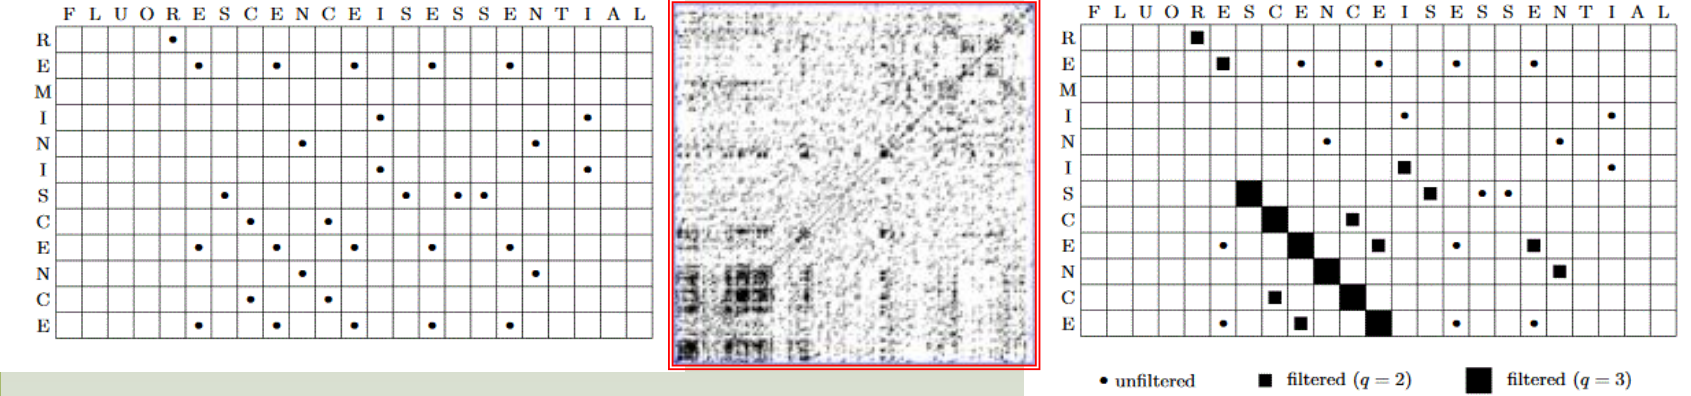
\includegraphics[width = \textwidth]{figs/dotmatrix.png}
\end{figure}

\item Puntuar la diagonal con los matches de los k-meros, identificando las 10 mejores diagonales.

Sobre el ejemplo, la matriz dot serían los puntos. Se coge como referencia la diagonal principal. Sobre ella, se realizan los desplazamientos positivos (hacia abajo) y negativos (hacia arriba). Los matches que se encuentran son los puntos que caen en las celdas de la diagonal. 
\begin{figure}[h]
\centering
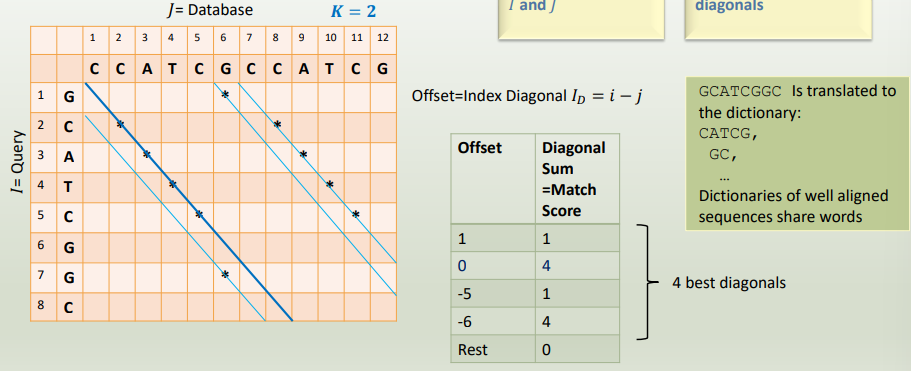
\includegraphics[width = \textwidth]{figs/diagonal-sums.png}
\end{figure}

\item Volver a puntuar regiones iniciales con una matriz de sustitución (PAM o BLOSUM).

Cada diagonal de puntuación alta elegida en el paso anterior se vuelve a puntuar según una matriz de puntuación (es decir, PAM). Esto se hace para encontrar subregiones con identidades más cortas que k. Los extremos de la diagonal que no coinciden se recortan. El parámetro más crítico en la comparación de secuencias es la elección de una matriz de puntuación.

\item Unir las regiones utilizando gaps, penalizándolos
\begin{figure}[h]
\centering
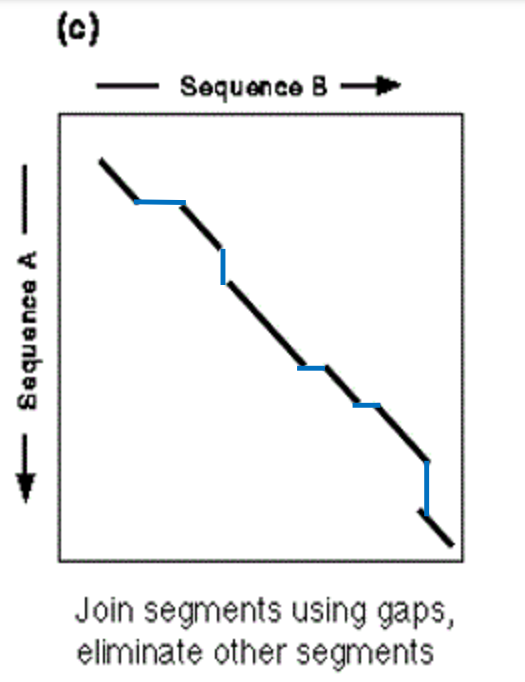
\includegraphics[width = 0.3\textwidth]{figs/join-segments.png}
\end{figure}

\item Utilizar programación dinámica para encontrar un alineamiento final.
\begin{figure}[h]
\centering
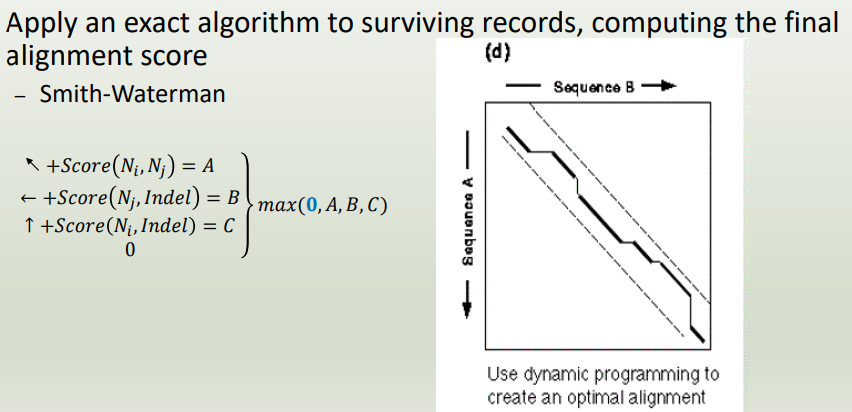
\includegraphics[width = 0.3\textwidth]{figs/final-fasta.png}
\end{figure}
\end{enumerate}

\paragraph{Evaluar la significancia del alineamiento}
Cuando se detecta similitud entre secuencias, hay dos posibilidades: que se deba al azar o debido a la evolución de un ancestro común (y por tanto una función similar). Por ello, se busca obtener una medida universal para inferir homología. ¿Qué diferencia hay entre el resultado de una coincidencia aleatoria y el de una coincidencia entre secuencias no relacionadas? Dado un conjunto de secuencias no relacionadas con la consulta (o un conjunto de secuencias aleatorias), ¿cuál es la probabilidad de encontrar una coincidencia con la misma puntuación de alineación por azar?
En una típica búsqueda actual en bases de datos, una proteína de longitud 250 podría ser comparada con una base de datos de proteínas de 50.000.000 de residuos totales.

Hay distintas medidas para ver la significancia estadística:
\begin{itemize}
\item \textbf{p-valor:} la probabilidad de que al menos una secuencia produzca la misma puntuación por azar. $P_{value} (S) = P(x \geq S)$, siendo S la puntuación y x la secuencia.

\item \textbf{E-valor:} número esperado de secuencias que producirán la misma o mejor puntuación por azar. Es la corrección de los p-valores para pruebas múltiples: $E_{value}(S) = P_{value} \cdot length.database \cdot length.query$

El valor E disminuye exponencialmente a medida que aumenta la puntuación (S) que se asigna a una coincidencia entre dos secuencias. Esto se debe a que, como la secuencia es más larga, hay más probabilidad de que se den matches. El valor E depende del tamaño de la base de datos (N) y del sistema de puntuación utilizado (es decir, PAM150, BLOSUM62). El valor E (asociado a una puntuación S) es el número de alineamientos distintos, con una puntuación equivalente o mejor que S, que se espera que se produzcan en una búsqueda en una base de datos por azar. Cuanto menor sea el valor E, más significativa será la puntuación. Como norma general:
\begin{itemize}
\item $Escore < 10^{-6}$: estadísticamente significativo
\item $10^{-6} < Escore < 10^{-3}$: se debe revisar.
\item $10^{-3} < Escore$: no significativo.
\end{itemize}

$$E = k \cdot m \cdot N |cdot e^{-\lambda S}$$
siendo:
\begin{itemize}
\item m: tamaño de la secuencia query
\item N: tamaño de la base de datos
\item k: constante estadística
\item $\lambda$: constante para ajustar la matriz de puntuación
\item S: puntuación de un high-scoring segment pair
\end{itemize}

\item \textbf{z-score:} mide cuántas desviaciones estándar hay por encima de la media de la distribución de la puntuación.
$$Z_{score} = \frac{S - \mu_S}{\sigma_S}$$

Se generan alineamientos aleatorios y se calcula su puntuación. Con eso, se calcula la media y la desviación estándar de las puntuaciones aleatorias, de forma que después se pueda calcular la desviación de la puntuación actual con la media de las puntuaciones aleatorias. La probabilidad de un z-score se denomina como e-valor.
\end{itemize}

\paragraph{Ejemplo: Retinoblastoma (RBP) vs $\beta$-lactoglobulina}
La segunda secuencia se aleatoriza 100 veces, permutando aleatoriamente («Barajando») las posiciones que ocupan los aminoácidos (manteniendo por tanto la longitud de la secuencia y la composición de aminoácidos). Cada secuencia aleatoria se alinea con la primera y se obtienen 100 puntuaciones «aleatorias». Es de esperar que la puntuación real sea mucho mayor que las 100 puntuaciones «aleatorias».
\begin{figure}[h]
\centering
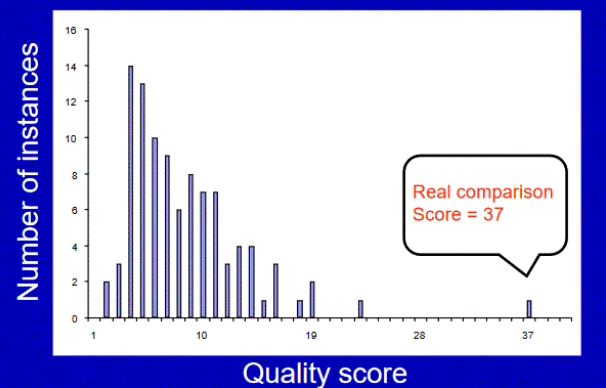
\includegraphics[width = 0.5\textwidth]{figs/shuffling.png}
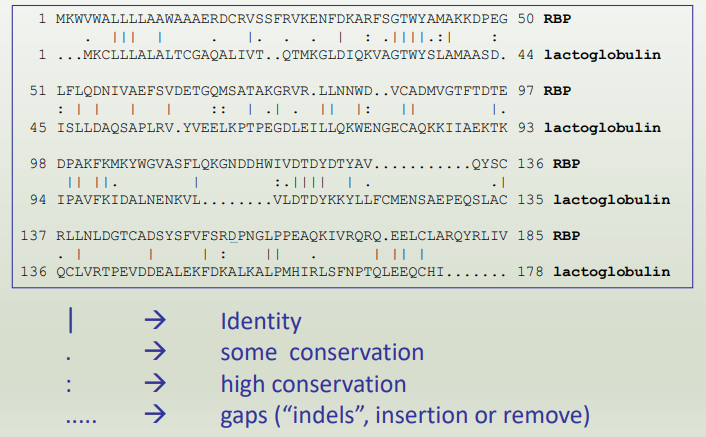
\includegraphics[width = 0.6\textwidth]{figs/alignment-ex.png}
\end{figure}

%06/03 - Ana
\subsubsection{BLAST}
El programa Basic Local Alignment Search Tool (BLAST) se utiliza ampliamente para alinear secuencias. El concepto básico es que:
\begin{itemize}
\item cuanto mayor sea el número de segmentos similares entre dos secuencias, y
\item cuanto mayor sea la longitud de los segmentos similares, menos diferentes son las secuencias y, por tanto, más relacionadas genéticamente (homólogas) es probable que estén
\end{itemize}

BLAST no garantiza el alineamiento óptimo al ser un método heurístico. Tiene un preprocesamiento en el que se crea una tabla de búsqueda de todos los k-meros. Los pasos son:
\begin{enumerate}
\item \textbf{Identificar semillas:} encuentra todos los substrings de longitud k en la secuencia de búsqueda que también está en la base de datos mediante la tabla de búsqueda.
\item \textbf{Extensión de semilla:} cada semilla se extiende hacia ambos lados hasta que la puntuación de alineamiento caiga por debajo de un umbral. Hay dos formas de extensión: sin huecos (solo se extiende con match o missmatch) o con huecos (se permite extender con match, missmatch o un número limitado de gaps).
\item \textbf{Registrar} todos los alineamientos locales que superen un determinado umbral estadístico. 
\item \textbf{Clasificar y ordenar} todos los alineamientos locales en orden ascendente del E-valor.
\end{enumerate}

\begin{figure}[h]
\centering
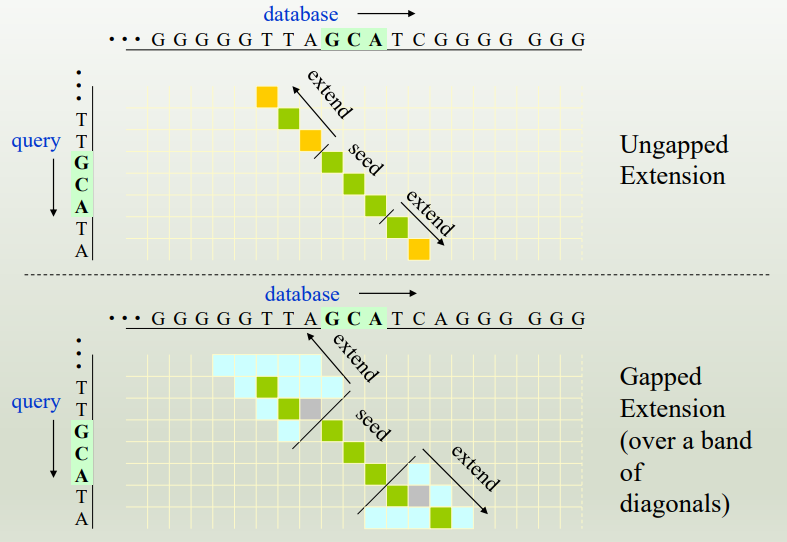
\includegraphics[width = 0.8\textwidth]{figs/blast.png}
\end{figure}

Si se tratara simplemente de comparar dos secuencias cualesquiera para ver si son homólogas, Smith-Waterman sería el método a elegir. FASTA y BLAST se utilizan en búsquedas de homólogos en grandes bases de datos: «Tengo una proteína/secuencia y quiero preguntar si está relacionada con algo de lo que se sepa algo». BLAST y FASTA son tan rápidos en parte porque empiezan buscando «palabras» cortas que coincidan exactamente y construyen un alineamiento más largo a partir de estas palabras. Como contrapartida a la ventaja de la velocidad, es posible que se pasen por alto algunas homologías.

\subsection{Alineamiento múltiple de secuencias (MSA)}
Hemos visto cómo comparar una secuencia con otra (alineamiento de pares) y con muchas otras en una base de datos (muchos pares de secuencia, es decir, BLAST). Ahora veremos cómo comparar múltiples secuencias simultáneamente, no de dos en dos. El alineamiento múltiple ilustra las relaciones entre dos o más secuencias.

Un alineamiento múltiple es una colección de tres o más secuencias de aminoácidos o nucleótidos parcial o completamente alineadas. El objetivo del análisis de secuencias múltiples es colocar en la misma columna las posiciones homólogas de secuencias homólogas.

\subsubsection{Alineamiento múltiple como generalización del alineamiento por pares}
En cuanto a la alineación por pares, el objetivo es encontrar el alineamiento que maximice alguna función de puntuación. Un alineamiento de este tipo se puntúa mediante la puntuación de la suma de pares (SP) o mediante la puntuación basada en la entropía (mínima).

\paragraph{Puntuación de suma de pares (SP)}
Considera todos los pares de letras de cada columna y suma las puntuaciones utilizando las matrices PAM o BLOSUM como matrices de puntuación. Esto no es un sistema de puntuación perfecto, ya que no hay ninguna justificación teórica biológica para la puntuación. 

\paragraph{Puntuación basada en entropía}
La entropía se calcula como el sumatorio negativo de la probabilidad de las letras con el logaritmo en base 2 de la probabilidad. Como la entropía es el desorden, la mejor puntuación sería la entropía más baja.

Estas puntuaciones se basan en las posiciones del alineamiento, y posteriormente se puede sumar la puntuación de todas las columnas para sacar la puntuación del alineamiento completo. 

Hay distintos tipos de alineamiento múltiple de secuencia:
\begin{itemize}
\item Programación dinámica: se puede aplicar al alineamiento de cualquier número de secuencias. Computa un alineamiento óptimo para una función de puntuación. No obstante, tiene un tiempo de computación grande de $O(n^k)$, siendo n la longitud de la secuencia y k el número de secuencias que se quieren alinear.
\item Métodos heurísticos:
\begin{itemize}
\item Métodos progresivos: CLUSTAL W, T-Coffee
\item Métodos iterativos: Muscle, MAFFT
\item Modelos ocultos de Markov: CLUSTAL Omega
\end{itemize}
\end{itemize}

\end{document}
